%!TEX root = ../thesis.tex
\chapter{Methodology}
\label{ch:methodology}
\begin{figure}[htbp]
    \centering
    \includesvg[width=\textwidth]{images/Ablaufdiagramm_white}
    \caption[Flowchart for workflow]{Flowchart for workflow. The VEDAI dataset is first used to investigate the differences between \acrshort{abb} and \acrshort{obb}, with the channel permutation experiments based on the respective better bounding box format. In the next step, a self-trained model based on the DOTA dataset is used as a pre-trained model. The permutation experiments based on this model comprise five different channel combinations and, optionally, the inclusion of NDVI in combination with several true colour channels (Own representation).}
    \label{fig:Flowchart}
\end{figure}

% \begin{itemize}
%     \item Methods und Implementierung zusammenlegen
%     \item Mein Vorschlag neuer Reihenfolge
%     \item 4.3 Database
%     \item 4.2 YOLOv9
%     \item 5.3 Python Packages
%     \item 5.1 Preproc
%     \item 4.1 (Herausforderungen Preproc)
%     \item 6.1 Results 5 Folds Cross Validation
%     \item 4.4 Palma
%     \item 5.2 Bash Scripte
%     \item 
% \end{itemize}
% \todo{vollständig diesen Absatz überarbeiten}



% Die methodische Vorgehensweise dieser Arbeit ist im zugehörigen Flowchart dargestellt\todo{Referenz zum Flowchart einfügen}. Als Datengrundlage dient das \acrshort{VEDAI}-Datenset, auf dessen Basis zunächst eine Entscheidung zwischen axis-aligned und oriented Bounding Boxes getroffen wird. Da aktuelle Versionen des \acrshort{YOLO}-Frameworks grundsätzlich mit beiden Formaten umgehen können, erfolgt die Auswahl anhand ihrer jeweiligen Eignung für die Aufgaben der Objekterkennung und -lokalisierung.

% Im Anschluss wird der \Acrfull{DOTA} genutzt, um ein vortrainiertes Modell zu erzeugen, das als Ausgangspunkt für das Training mit Kanalpermutationen dient. Abhängig von der zuvor gewählten Bounding-Box-Variante wird auch die Channel Permutation mit diesem Format durchgeführt.

% Im Rahmen der Experimente werden verschiedene Kanalpermutationen (s. Tab. \ref{tab:perm}) getestet.


Die methodische Vorgehensweise dieser Arbeit ist im zugehörigen Flowchart (s. Fig. \ref{fig:Flowchart}) dargestellt. Das \acrshort{VEDAI}-Dataset wird zuerst zur Untersuchung der Unterschiede zwischen \acrshort{abb} und \acrshort{obb} verwendet, wobei die Experimente zu den Kanalpermutationen auf dem jeweils besseren Bounding-Box-Format basieren. Im nächsten Schritt kommt als vortrainiertes Modell ein selbst trainiertes Modell auf Basis des DOTA-Datensatzes zum Einsatz. Die darauf aufbauenden  Permutationsexperimente umfassen fünf verschiedene Kanalkombinationen sowie optional die Einbeziehung von NDVI in Kombination mit mehreren Echtfarbkanälen.

Im folgenden Abschnitt wird die Methodik dieser Arbeit beschrieben. Zunächst wird die Datengrundlage anhand der verwendeten Datensätze erläutert. Darauf aufbauend werden die eingesetzten \acrshort{YOLO}-Versionen vorgestellt. Im Anschluss folgt die Implementierung, bestehend aus den verwendeten Python-Packages sowie einer Beschreibung des Programmcodes, welcher auf Github \cite{Github_timo} zur Verfügung gestellt wird. Danach werden die zentralen Herausforderungen im Preprocessing dargestellt. Anschließend werden die Ergebnisse der 6-Fold-Cross-Validation präsentiert, wobei eigene Folds erstellt wurden, die für alle Experimente mit \acrshort{abb}, \acrshort{obb} sowie den Permutationen (s. Tab. \ref{tab:perm}) genutzt wurden. Abschließend wird die Hardware beschrieben, auf der die Experimente durchgeführt wurden, nämlich der \acrlong{HPC} \acrshort{PALMA}, sowie die dort ausgeführten Bash-Skripte mit den für \acrshort{YOLO} verwendeten Hyperparametern.  

% \begin{itemize}
%     \item Im folgenden Abschbnitt wird die Methodik beschrieben
%     \item Erst wird die Datengrundlage anhand der verwendeten Datensätze erläutert
%     \item Dann die genutzten \acrshort{YOLO} Versionen
%     \item dann die Implementierung in Form der genutzten Python Packages und einer Beschreibung des Programmcodes
%     \item dann die Herausforderungen beim Preprocessing
%     \item dann Ergebnisse (Verteilung) der 5 Fold Cross Validation, (eigene Folds erstellt, die als für alle Experimente (\acrshort{abb} und \acrshort{obb}, sowie die Permutation genutzt wurden}))
%     \item Zuletzt die Hardware auf der die Experimente liefne (\acrlong{HPC} \acrshort{PALMA}) und die auf \acrshort{PALMA} laufenden Bash scripte mit den für \acrshort{YOLO} genutzten Hyperparametern
% \end{itemize}

\begin{table}[h!]
\centering
\begin{tabular}{l|c|c|c|c|c}
\textbf{Permutation} & \textbf{Red (R)} & \textbf{Green (G)} & \textbf{Blue (B)} & \textbf{Infrared (IR)} & \textbf{NDVI} \\
\hline
\acrshort{RGBIR}    & x & x & x & x &   \\
\acrshort{IRGB}     &   & x & x & x &   \\
\acrshort{RIRB}     & x &   & x & x &   \\
\acrshort{RGB}      & x & x & x &   &   \\
\acrshort{RGIR}     & x & x &   & x &   \\
\acrshort{RGBNDVI}  & x & x & x &   & x \\
\acrshort{GBNDVI}   &   & x & x &   & x \\
\end{tabular}
\caption{Channel permutations represented by included channels (x = channel present).}
\label{tab:perm}
\end{table}
% Die Evaluation der Ergebnisse erfolgt auf Basis der \acrshort{mAP}$_{50\text{-}95}$-Werte, welche eine standardisierte Bewertung der Modellleistung über verschiedene \Acrshort{IoU}-Schwellen hinweg ermöglichen. 

% Zuletzt wurde eine Ablationsstudie unter Verwendung der Kanäle \Acrfull{R}, \Acrfull{G}, \Acrfull{B}, \acrshort{IR} und \acrshort{NDVI} durchgeführt.

% \begin{itemize}
%     \item Im Flowchart (\todo{Ref einfügen}) ist die Methodik dieser Thesis zu erkennen
%     \item VEDAI Dataset als Grundlage; erste Entscheidung zwischen Axis Aligned und ORiented Bounding Boxen (YOLO kann mit beiden Formaten je nach VErsion umgehen, schauen welche Form besser geeignet für Objekterkennung und -detektierung ist)
%     \item dann Training des DOTA Datensatzes als Pretrained Model für die Channel Permutation
%     \item Je nach Bounding Box Evaluationsergebnis wird dann die Channel Permutation mit dieser BB Art durchgeführt. Folgende Permutationen werden berechnet: RGBIR; IRGB; RIRB; RGB, RGIR und sowie als Erweiterung optional RGBNDVI, GBNDVI
%     \item Anhand der Map50-95 Werte kann dann die Evaluation erfolgen
% \end{itemize}
\section{Database}
Die Datenbasis umfasst 2 Datensätze, die annotierte Luft- und Satellitenbildern enthalten. Das \acrshort{DOTA} Dataset wurde genutzt, um ein vortrainiertes Modell zu erzeugen, das als Ausgangspunkt für das Training mit Kanalpermutationen dient, während das \acrshort{VEDAI} Dataset mit der in Sec. \ref{sec_5Fold_CV} beschriebenen Verteilung für die Permutationsexperimente genutzt wurde.
\subsection{Vehicle Detection on Aerial Images (VEDAI) Dataset}
\label{subsec:VEDAI}

Das \Acrshort{VEDAI} Dataset \cite{vedai_web}  aus dem Jahr 2015 bietet sich als Datengrundlage an, da es hochauflösende Luftbilder enthält, die speziell für die Fahrzeugerkennung geeignet sind \cite{Razakarivony2015}. Es umfasst annotierte Daten, die Fahrzeuge in unterschiedlichen Szenarien, Größen und Orientierungen zeigen. Außerdem ist es ein Benchmark für die Detektion von sehr kleinen Objekten. Das Dataset enthält sowohl \acrshort{RGB}-Bilder als auch multispektrale Daten, was es ideal für die Untersuchung der Auswirkungen zusätzlicher Kanäle wie \acrshort{IR} auf die Objekterkennung macht. Es sind mehr als 3700 Objekte in ungefähr 1200 Bildern annotiert. Diese Objekte sind in 9 Klassen (Ship, Camping Car, Car, Pickup, Plane, Tractor, Truck, Van und Vehicles) unterteilt und der Hintergrund der Objekte ist abwechslungsreich, was die Robustheit des trainierten Modelles erhöht \cite{Razakarivony2015}. \\
Die Auflösung der Bilder liegt bei 12.5 cm \texttimes 12.5 cm pro Pixel, was ausreichend ist um einzelne Fahrzeuge zu erkennen. Die Bilder mit einer Größe von 1024 \texttimes 1024 Pixeln sind bei einer Befliegung im Jahr 2012 in US Amerikanischen Bundesstaat Utah aufgenommen worden \cite{Razakarivony2015}. Beispielbilder für jede Klasse sind in den Abbildungen \ref{fig:aab_obb_example_pics}, \ref{fig:perm_exp_example_pics} und \ref{fig:ablation_example_pics} zu sehen.



\subsection{Dataset for Objectdetection in Aerial Images (DOTA) 1.5}
\label{subsec:DOTA}
Das \Acrfull{DOTA} eignet sich aufgrund seiner Vielfalt an Klassen und seiner domänenspezifischen Ausrichtung besonders gut als Grundlage für das Pretraining in den Permutationsexperimenten. Der Datensatz enthält eine große Anzahl annotierter Objekte aus verschiedenen Kategorien, die in hochauflösenden Satellitenbildern enthalten sind. Die Bildauflösungen im \acrshort{DOTA}-Datensatz variieren stark und reichen von 800~$\times$~800 bis hin zu 20\,000~$\times$~20\,000 Pixeln. Dabei umfasst der Datensatz sowohl \acrshort{RGB}-Bilder als auch Graustufenbilder, die den panchromatischen Kanal der GF2- und JL1-Satelliten darstellen. Die Bilder stammen aus verschiedenen Quellen, unter anderem von Google Earth sowie weiteren kommerziellen und institutionellen Anbietern.

Für das Training in dieser Arbeit wurden alle 16 verfügbaren Klassen des DOTA-Datensatzes berücksichtigt. Besonders relevant für die anschließenden Experimente sind die Klassen \textit{Large Vehicle}, \textit{Small Vehicle}, \textit{Plane} und \textit{Ship}, da sie eine hohe Bedeutung für die Objekterkennung im urbanen und infrastrukturellen Kontext besitzen.

Das Training wurde mit dem Modell \acrshort{YOLO}v9u über 1500 Epochen durchgeführt, wobei eine \textit{Patience} von 150 verwendet wurde. Alle weiteren Hyperparameter wurden analog zu den in Tabelle~\ref{tab:hyperparameters} dargestellten Einstellungen gewählt. Die erzielten Ergebnisse zeigen einen mittleren \acrshort{mAP}50-95 von ca. 0,42, was angesichts der großen Anzahl an Bildern und Klassen als zufriedenstellender Wert zu bewerten ist. Es ist kein Overfitting erkennbar, und die Precision-Werte sind insgesamt gut. Die Metriken des Trainingsverlauf sind in Abbildung~\ref{fig:DOTA_train_values} und Beispielklassen in Fig. \ref{fig:DOTA_exClasses} dargestellt.





\section{YOLOv9}
\label{sec:yolov9}

%##########################################################################
%##########################################################################
%##########################################################################
%##########################################################################
%##########################################################################
%##########################################################################
%##########################################################################
%##########################################################################
%##########################################################################

\begin{figure}[ht]
  \centering
  
  \begin{subfigure}{0.32\textwidth}
    \centering
    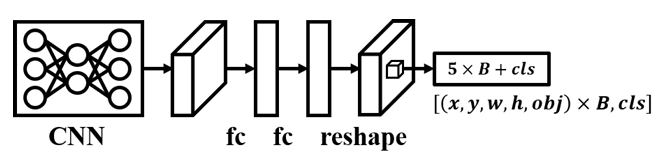
\includegraphics[width=\linewidth]{images/013Methods/yolov1_arch.png}
    \caption{v1}
    \label{subfig_yolov1}
  \end{subfigure}
  \hfill
  \begin{subfigure}{0.32\textwidth}
    \centering
    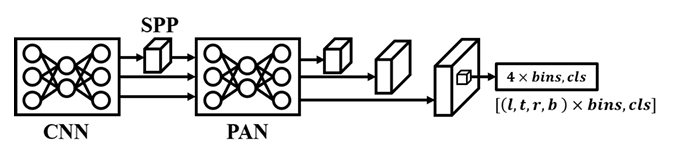
\includegraphics[width=\linewidth]{images/013Methods/yolov8_arch.png}
    \caption{v8}
    \label{subfig_yolov8}
  \end{subfigure}
  \hfill
  \begin{subfigure}{0.32\textwidth}
    \centering
    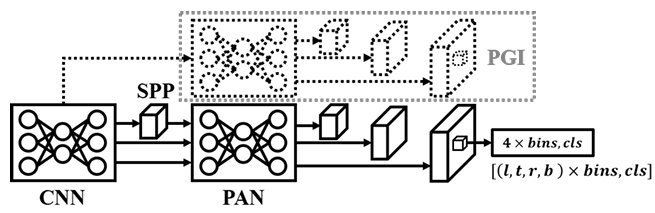
\includegraphics[width=\linewidth]{images/013Methods/yolov9_arch.png}
    \caption{v9}
    \label{subfig_yolov9}
  \end{subfigure}
  
  \caption{Different YOLO Architectures}
\end{figure}



% \begin{itemize}
%     \item Weiterentwicklung von YOLO zeigt sich in dem Unterschied zur Archtektur von YOLOv1 über v8 bis zu v9
%     \item yolov1 kann durch die One Stage Methode eine große Anzahl von Parametern und Berechnungen vermeiden, da Sie durch die   \acrshort{FCL} in der zweiten Schicht erzeugt werden
%     \item yolov8 basiert auf yolov5 und nimmt azhlreiche optimierungen hinzu. Die \acrfull{ELAN} Integration aus YOLOv7 wird um eine zusätzliche Residual Connection erweitert und der Decoder, basierend auf YOLOv6, bleibt identisch
%     \item Yolov8 hat eine Verbesserung der Trainingsleistung von 30\% udn bietet verschiedene Möglichkeiten um nachgelagerte Aufgaben des Downstreamdetectors zu ermöglichen (wie segment anything, instance segmentation, pose estimation, multiple object tracking)
%     \item yolov9 kann durch die \acrshort{PGI} Integartion das Problem vermeiden, dass wichtige Informationen bei der oberflächlichen Netzebene verloren gehen. PGI sorgen für eine robustere Leistung ,weil die Originalinformaitonen maximal tief beibehalten werden
% \end{itemize}

Die Entwicklung von \acrshort{YOLO} über die verschiedenen Versionen hinweg zeigt deutliche Fortschritte. Während \acrshort{YOLO}v1 (s. Fig. \ref{subfig_yolov1}) durch die One-Stage-Methode eine große Anzahl an Parametern und Rechenaufwand einsparen konnte, indem Vorhersagen durch die \acrshort{FCL} in der zweiten Schicht erzeugt wurden, baut \acrshort{YOLO}v8 (s. Fig. \ref{subfig_yolov8}) auf \acrshort{YOLO}v5 auf und integriert zahlreiche Optimierungen \cite{Wang2024_yolo_review}. Dazu gehört die \acrfull{ELAN}-Integration aus \acrshort{YOLO}v7, die um eine zusätzliche Residual Connection erweitert wurde, während der Decoder auf \acrshort{YOLO}v6 basiert und unverändert bleibt. Diese Version zeigt zudem eine Verbesserung der Trainingsleistung um etwa 30\% und ermöglicht verschiedene nachgelagerte Aufgaben wie Segmentierung, Instanzsegmentierung, Posenabschätzung und Multiple-Object-Tracking. \acrshort{YOLO}v9 (s. Fig. \ref{subfig_yolov9}) integriert schließlich \acrshort{PGI}, um zu verhindern, dass wichtige Informationen auf oberflächlicher Netzebene verloren gehen. \acrshort{PGI} sorgen für eine robustere Leistung, indem die Originalinformationen maximal tief beibehalten werden \cite{Wang2024_yolo_review}.


Die zentralen Stärken von \acrshort{YOLO}v9 liegen in seiner hohen Verarbeitungsgeschwindigkeit sowie der präzisen Objekterkennung, wodurch eine effiziente Analyse großer Datensätze ermöglicht wird. 


Die Varianten \acrshort{YOLO}v9u und \acrshort{YOLO}v9e unterscheiden sich primär hinsichtlich des verwendeten Labelformats. \acrshort{YOLO}v9e verwendet ein normiertes Koordinatensystem:
\hypertarget{eq:yolov9}{}
\begin{equation}
x_\text{norm} = \frac{x_\text{pixel}}{w_\text{image}},\;\;
y_\text{norm} = \frac{y_\text{pixel}}{h_\text{image}},\;\;
w_\text{norm} = \frac{w_\text{box}}{w_\text{image}},\;\;
h_\text{norm} = \frac{h_\text{box}}{h_\text{image}}
\end{equation}
\label{Eq:yolov9}

\hypertarget{eq:yolov9u}{}
\acrshort{YOLO}v9u hingegen verwendet ein Polygonformat:
\begin{equation}
(\text{class\_index},\ x_1, y_1, x_2, y_2, x_3, y_3, x_4, y_4).
\end{equation}

%\todo{passt das so rein? überhaupt sinnvoll? verstehen und so...}
% Die YOLOv9-Architektur nutzt einen tiefen, GELAN-basierten Backbone mit umfangreicher Feature-Fusion (\texttt{CBLinear}, \texttt{CBFuse}) und Downsampling-Blöcken (\texttt{ADown}), wodurch klassische achsenausgerichtete Bounding-Boxes über den \texttt{Detect}-Layer erzeugt werden. YOLOv9u hingegen verfolgt einen schlankeren Aufbau mit flacherem Backbone, reduzierter Tiefe der \texttt{RepNCSPELAN4}-Blöcke und minimaler Backbone-Fusion. Die Downsampling-Stufen erfolgen hier über einfache Convolutionen, und die Detektion zielt auf orientierte Bounding-Boxes (\texttt{OBB}) ab. Somit besteht ein klarer Trade-off zwischen Modellkomplexität und Effizienz sowie spezialisierter Detektionsfähigkeit.


% Dieses unterschiedliche Labelformat reflektiert die jeweiligen Stärken der Modelle: \texttt{YOLOv9e} ist auf axis-aligned Bounding Boxes optimiert, während \texttt{YOLOv9u} die präzise Darstellung orientierter Objekte ermöglicht.


% \begin{itemize}
%     \item Beide Varianten \acrshort{YOLO}v9u und \acrshort{YOLO}v9e unterscheiden sich durch das genutzte Labelformat
%     \item yolov9e: normalized_x = x_pixel / image_width normalized_y = y_pixel / image_height  normalized_width = box_width_pixel / image_width  normalized_height = box_height_pixel / image_height
%     \item yolov9u: class_index x1 y1 x2 y2 x3 y3 x4 y4
% \end{itemize}

%\todo{Unterschiedliches Labelformat beider Varianten erklären? und bei Implementierung auf Abschnitt verweisen?}

\subsection{YOLOv9u by Wong Kin Yiu}
\label{subsec:yolov9u}

Die Implementierung von \acrshort{YOLO}v9u basiert auf der Version \acrshort{YOLO}v8.1.23 \cite{yolo_v9u_github}, um die ursprüngliche \acrshort{YOLO}v9 Version um diverse nachgelagerte Aufgaben zu erweitern. Hierzu zählen Instanzsegmentierung, orientierte Objekterkennung, Posenabschätzung, Bildklassifikation sowie transformerbasierte Objekterkennung \cite{wang2024}, wobei mit \acrshort{YOLO}v8 als Basis ein \textit{Detect}-Layer integriert wird, der die Vorhersage orientierter \acrshort{BB} ermöglicht. In der vorliegenden Arbeit wird \acrshort{YOLO}v9u eingesetzt, da diese als Open-Source-Variante verfügbar ist und die zugrundeliegende Methodik durch das veröffentlichte Paper dokumentiert wurde \cite{wang2024_sapkota}. Das Modell \acrshort{YOLO}v9e wird von Ultralytics bereitgestellt, jedoch ohne begleitende wissenschaftliche Veröffentlichung, sodass dessen Aufbau und methodische Grundlagen nicht nachvollziehbar dokumentiert sind \cite{ultralyics_2023}.

 


% Die Implementierung von \texttt{YOLOv9u} basiert auf der Version \texttt{YOLOv8.1.23}\cite{yolo_v9u_github} und stellt eine umfassende Weiterentwicklung der \acrshort{YOLO}-Architektur im Vergleich zu \acrshort{YOLO}v8 durch den Einsatz von \acrshort{PGI} und \acrshort{GELAN} dar. Der Einsatz von \acrshort{PGI} ermöglicht die vereinfachte Anwenung neuer leichtgewichtiger Netzwerkarchitekturen und löst das Problem der Verwendung von Deep Supervision nur für extrem tiefe neuronale Netze. Das Nutzen von des von \citeauthor{wang2024_sapkota} entworfenen \acrshort{GELAN} kann durch die Verwendung der herkömmlichen Faltungen eine höhere Parameterauslastung erreichen. Dies bietet auc hVorteile für die Geschwindigkeit und Genauigkeit. Neben der klassischen Objekterkennung unterstützt \texttt{YOLOv9u} durch die Basis von \acrshort{YOLO}v8 zusätzliche Aufgaben wie Instanzsegmentierung, orientierte Objekterkennung, Posenabschätzung, Bildklassifikation sowie transformerbasierte Objekterkennung\cite{wang2024}. Damit bietet das Modell eine erweiterte Funktionalität gegenüber früheren \acrshort{YOLO}-Versionen, sowie der originalen \acrshort{YOLO}v9-Version, und eignet sich insbesondere für komplexe Szenarien mit mehreren Aufgabenstellungen innerhalb eines Frameworks. Diese Version wird genutzt, da sie \acrlong{obb} unterstützt.

\subsection{YOLOv9e by Ultralytics}
\label{subsec:yolov9e}

Die \acrshort{YOLO}v9-Modellreihe von Ultralytics umfasst mehrere Varianten, die sich in Bezug auf Modellgröße, Genauigkeit und Rechenkomplexität unterscheiden. Alle Varianten integrieren die von \citeauthor{wang2024_sapkota} entwickelten \acrshort{PGI}- und \acrshort{GELAN}-Architekturen und unterstützen zudem die Verarbeitung von \acrshort{abb}. Die Bandbreite reicht von der kompakten \texttt{YOLOv9t}-Variante mit einer Eingabebildgröße von $640 \times 640$ Pixeln, 2 Millionen Parametern und 7{,}7 \acrshortpl{GFLOP} bis hin zur leistungsstärksten \acrshort{YOLO}v9e-Variante mit 58{,}1 Millionen Parametern und 192{,}5 \acrshortpl{GFLOP} (siehe Tabelle~\ref{tab:yolov9-models}).  

Aufgrund der höchsten erzielten Genauigkeit (\acrshort{mAP}50-95 = 55,6) sowie der höchsten Rechenkapazität wurde das \texttt{YOLOv9e}-Modell für alle Experimente mit axis-aligned Bounding Boxes verwendet. Die Wahl dieser Variante erfolgte mit dem Ziel, die maximale Detektionsleistung im Rahmen der Evaluierung sicherzustellen. Zudem wird diese Version genutzt, da sie die Verarbeitung von \acrlong{abb} unterstützt.

% \subsection{Differences YOLOv9u and YOLOv9e}
% \todo{wirklich nötig?}
% Die YOLOv9-Architektur und ihre Variante YOLOv9u unterscheiden sich in mehreren wesentlichen Aspekten, die sowohl die Modellkomplexität als auch die Detektionsfähigkeiten betreffen. YOLOv9 verwendet einen tiefen, GELAN-basierten Backbone, der mehrere Feature-Fusionsblöcke (\texttt{CBLinear}, \texttt{CBFuse}) sowie Downsampling-Blöcke (\texttt{ADown}) integriert. Diese Struktur ermöglicht eine intensive Mischung von Merkmalen über unterschiedliche Auflösungsebenen hinweg und unterstützt dadurch die Erkennung von Objekten in verschiedenen Skalen. Der Head von YOLOv9 kombiniert Features auf mehreren Ebenen mittels Upsampling und Concat-Operationen und erzeugt klassische, achsenausgerichtete Bounding-Boxes über den finalen \texttt{Detect}-Layer.  

% Im Gegensatz dazu verfolgt YOLOv9u einen kompakteren und effizienteren Aufbau. Der Backbone ist flacher und verzichtet weitgehend auf interne Feature-Fusionen im Vergleich zu YOLOv9. Downsampling erfolgt hier über einfache Convolutional-Blöcke mit Stride 2, und die Tiefe der \texttt{RepNCSPELAN4}-Blöcke ist reduziert. Im Head werden die Features ebenfalls mittels Upsampling und Concat kombiniert, jedoch ohne die zusätzlichen Downsampling-Blöcke des Originals. Ein entscheidender funktionaler Unterschied besteht darin, dass YOLOv9u orientierte Bounding-Boxes (\texttt{OBB}) generiert, während YOLOv9 klassische Bounding-Boxes liefert.  

% Zusammenfassend lässt sich sagen, dass YOLOv9 eine komplexere und tiefere Architektur mit intensiver Feature-Fusion darstellt, die tendenziell eine höhere Genauigkeit bei klassischen Bounding-Boxes ermöglicht. YOLOv9u hingegen bietet eine schlankere, effizientere Struktur mit reduzierter Rechenlast und ist speziell für die Detektion orientierter Objekte optimiert. Die Wahl zwischen beiden Varianten hängt somit von den Anforderungen an Genauigkeit, Rechenaufwand und Art der zu detektierenden Objekte ab.


\begin{table}[h]
\centering
\begin{tabular}{l|c|c|c|c|c} % keine äußeren vertikalen Linien
\textbf{Model} & \textbf{Image Size} & \textbf{mAP$_{\text{val}}$ 50--95} & \textbf{mAP$_{\text{val}}$ 50} & \textbf{Parameters (M)} & \textbf{FLOPs (B)} \\
\hline
YOLOv9t & 640 & 38.3 & 53.1 & 2.0 & 7.7 \\
YOLOv9s & 640 & 46.8 & 63.4 & 7.2 & 26.7 \\
YOLOv9m & 640 & 51.4 & 68.1 & 20.1 & 76.8 \\
YOLOv9c & 640 & 53.0 & 70.2 & 25.5 & 102.8 \\
YOLOv9e & 640 & 55.6 & 72.8 & 58.1 & 192.5 \\
\end{tabular}
\caption{Comparison of YOLOv9 model variants in terms of accuracy and computational complexity at an input resolution of 640$\times$640 pixels. \cite{ultralyics_yolov9,wang2024_sapkota}}
\label{tab:yolov9-models}
\end{table}



%##########################################################################
%##########################################################################
%##########################################################################
%##########################################################################
%##########################################################################
%##########################################################################
%##########################################################################
%##########################################################################


\section{Programming Environment}
Die genutzte Programmiersprache ist Python. Die Scripte für den \acrshort{HPC} \acrshort{PALMA} wurden in Bash geschrieben.

\subsection{Python Packages}
Es wurden diverse Python Packages zur Implementierung genutzt, die im folgenden kurz beschrieben werden. 
\subsubsection{Computer Vision 2}
Ein Teil der "Open Source Computer Vision" Bibliothek ist \Acrfull{CV2} \cite{opencv_about}. Die aktuelle Version 4.12.0 wurde am 09.07.2025 veröffentlicht \cite{opencv_release}. \\
Die Bibliothek bietet Algorithmen und Funktionen zur Bild- und Videobearbeitung an, die in dieser Arbeit hauptsächlich dazu genutzt werden, die verschiedenen Kanäle zu neuen Bildern zu kombinieren. Hierbei ist zu beachten, dass \acrshort{CV2} Bilder als BGR (Blue, Green, Red) Farbkombination abspeichert, was zu Falschfarbdarstellungen einiger Abbildungen, die in RGB abgeildet werden, (wie Fig. \ref{fig:perm_exp_example_pics}) führen kann.
\subsubsection{Numpy}
Ein weiteres Open-Source Projekt ist NumPy, welches 2005 gegründet wurde, um numerische Operationen in Python zu implementieren \cite{numpy_about}. Die aktuelle Version ist 2.3.0 und wurde am 07.06.2025 veröffentlicht \cite{numpy_main_web}. \\
Mithilfe dieser Bibliothek kann eine zufällige Verteilung der Bilddaten auf die Folds realisiert werden, indem die eingelesene Bildliste einer zufälligen Permutation unterzogen wird. Darüber hinaus stellt die Bibliothek Funktionen zur Verfügung, mit denen sowohl die Berechnung und Reskalierung des \acrshort{NDVI}-Kanals als auch die Transformation der Bounding-Box-Koordinaten in das für das \acrshort{YOLO}-Framework erforderliche Format durchgeführt werden können. Zusätzlich ermöglicht sie die Umrechnung axis-aligned Bounding Boxes in oriented Bounding Boxes sowie die Flächenberechnung beider Bounding-Box-Typen.
\subsubsection{Scipy}
SciPy ist in der Version 1.16.0 am 22.06.25 veröffentlicht worden \cite{scipy-main}. Diese Bibliothek bietet Algorithmen für wissenschaftliche Berechnungen in Python an \cite{scipy-main}. Die Unterfunktion "ConvexHull" wird zur Flächenberechnung der oriented Bounding Boxen genutzt.
\subsection{Additional Python-Packages for data analysis}
Zur Analyse der Modelle wurden die folgenden Bibliotheken verwendet.
\subsubsection*{Matplotlib}
Die Bibliothek "Matplotlib" wurde in der Version 3.10.0 am 23.12.2024 veröffentlicht\cite{matplotlib}. Im Rahmen dieser Arbeit werden durch diese Erweiterung die Datenanalysen und die Ausgabe der Plots ermöglicht.
\subsubsection*{Seaborn}
"Searborn" ist in der Version 0.13.2 im Januar 2024 veröffentlicht worden \cite{seaborn}. Die Bibliothek ermöglicht das Erstellen von Grafiken, wie Boxplots, zur vereinfachten Datenanalyse.
\subsubsection*{pandas}
Die Bibliothek "pandas" ist ebenfalls ein Open Source Datenanalyse und -manipulierungstool. Die aktuelle Version 2.3.1 wurde am 07.07.2025 veröffentlicht. Die Bibliothek wird auch zur Datenanalyse in dieser Arbeit verwendet \cite{pandas}.

%!TEX root = ../thesis.tex
\chapter{Implementation}
\label{ch:implementation}




\section{Challenges Preprocessing}
Bei der Verarbeitung des VEDAI-Datensatzes traten mehrere technische Herausforderungen auf. 
Zunächst mussten die vorhandenen Label in das \acrshort{YOLO}v9-\acrshort{obb}-Format konvertiert werden, um mit dem gewählten Modell kompatibel zu sein. 
Dabei zeigte sich, dass ein kleiner Teil der Daten (7 von 3\,757 Instanzen) Koordinatenwerte aufwies, die außerhalb des zulässigen Bereichs lagen (d.\,h. kleiner als 0 (s. Fig. \ref{fig:smaller0}) oder größer als 1 (s. Fig. \ref{fig:higher1})) . 
Dieses Problem wurde durch den Einsatz von Exception Handling sowie durch Rundung der Werte auf den gültigen Wertebereich behoben. 

\begin{figure}[h]
    \centering
    \begin{subfigure}[b]{0.45\textwidth}
        \centering
        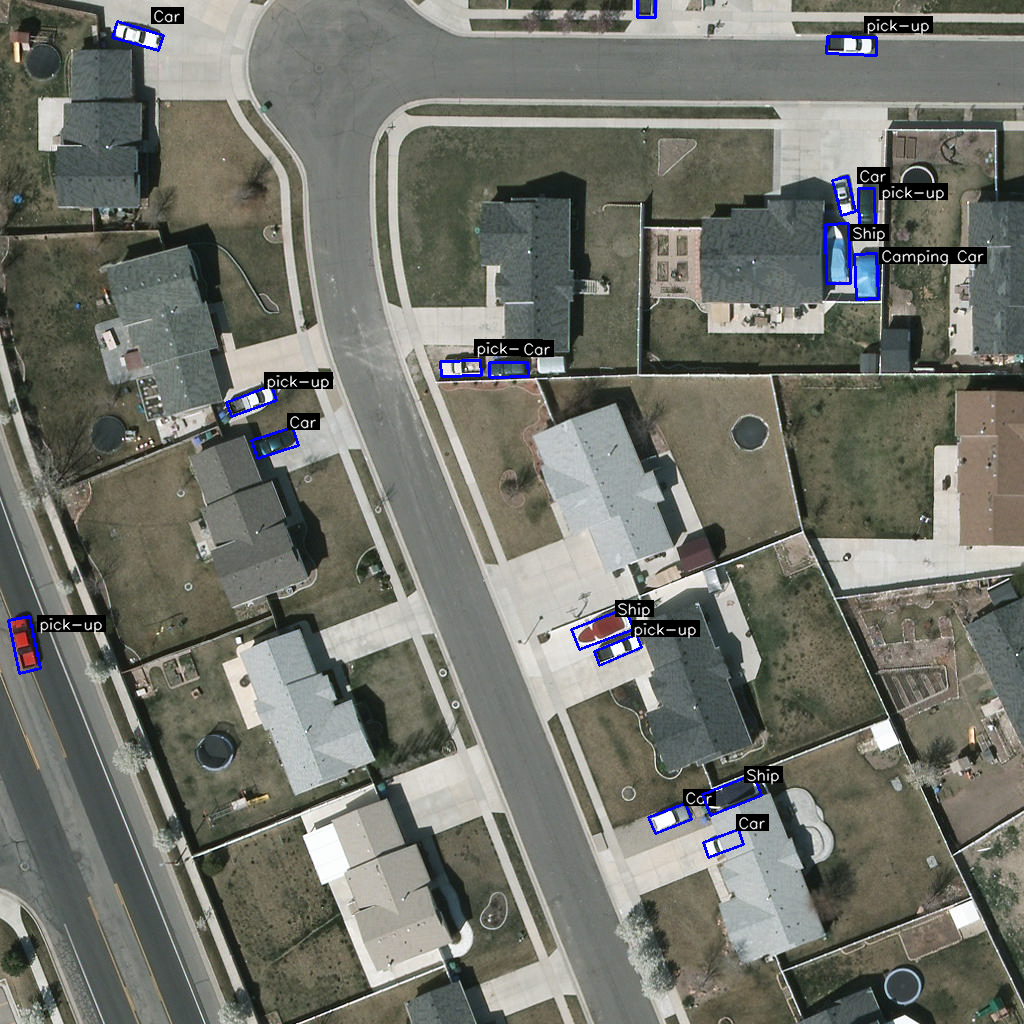
\includegraphics[trim={600pt 1000pt 350pt 0pt},clip,width=\textwidth]{images/bb_smaller0.png}
        \caption{Two Coordinate out of range and smaller 0}
        \label{fig:smaller0}
    \end{subfigure}
    \hfill
    \begin{subfigure}[b]{0.45\textwidth}
        \centering
        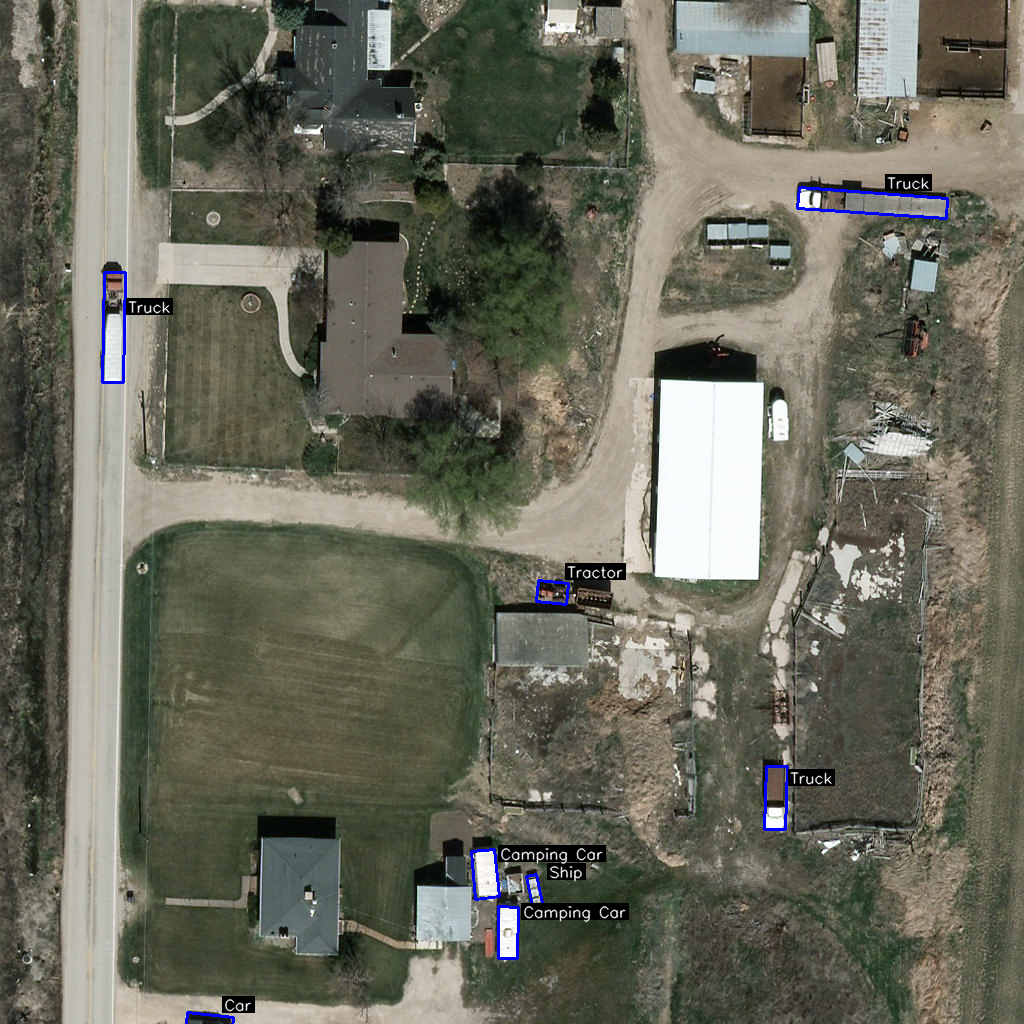
\includegraphics[trim={180pt 0pt 750pt 993pt},clip,width=\textwidth]{images/bb_higher1.png}
        \caption{Two Coordinates out ouf range and higher 1}
        \label{fig:higher1}
    \end{subfigure}
    \caption[Example for label coordinates outside of the image]{Example for label coordinates outside of the image (for full-sized Image see \ref{fig:example_coords_ooR_fs})}
    \label{fig:example_coords_ooR}
\end{figure}

% Da die von \citeauthor{Razakarivony2015} \cite{Razakarivony2015} verwendeten Folds nicht disjunkt waren, erhöhte sich das Risiko von Overfitting (s. Kap. \ref{subsec:overfitting}), sodass eigene Folds erstellt werden mussten (s. Kap. \ref{subsec:Fold_creation}), deren Verteilung im folgenden Abschnitt beschrieben wird. \todo{satz überarbeitne, doppelung}






\section{6-Fold-Cross-Validation}
\label{sec_5Fold_CV}

Um die Robustheit der Ergebnisse sicherzustellen und eine fundierte Vergleichbarkeit verschiedener Modelle zu ermöglichen, wurde in dieser Arbeit eine 6-Fold-Cross-Validation angewendet. Insbesondere wurde Wert darauf gelegt, die Evaluation nicht nur auf einem Teildatensatz durchzuführen, sondern eine Mehrfachteilung der Daten vorzunehmen, sodass Schwankungen durch unterschiedliche Trainings- und Validierungsaufteilungen minimiert werden.

Im Gegensatz zu den von \citeauthor{Razakarivony2015} \cite{Razakarivony2015} bereitgestellten Folds, deren Zusammenstellung identische Bilder gleichzeitig im Trainings- und Validierungssatz aufweist, wurden für diese Arbeit eigene, disjunkte Folds generiert. Letztere gewährleisten, dass keine Überlappungen zwischen Trainings- und Validierungsdaten existieren und somit die Gefahr von verfälschten Trainingsergebnissen durch Overfitting ausgeschlossen ist. Die genaue Methodik der Fold-Erstellung ist in Kapitel \ref{subsec:Fold_creation} beschrieben. 

Die Datenaufteilung erfolgte in sechs Folds (0-5): Fünf Folds (Fold 0 bis 4) wurden jeweils für Training und Validierung genutzt, während Fold 5 ausschließlich für abschließende Testzwecke reserviert blieb. Dadurch wurde erreicht, dass die finale Evaluation auf bisher ungesehenen, neutralen Daten stattfand.

Ein besonderes Augenmerk galt einer homogenen Verteilung der Objekte und Objektklassen über alle Folds hinweg. Jeder Fold umfasst zwischen 207 und 221 Bilder, darin enthalten sind jeweils drei bis sieben reine Hintergrundbilder ohne Objekte. Dies ermöglichte eine ausgewogene und repräsentative Bewertung der Modelle hinsichtlich aller vorkommenden Klassen. Die resultierende Klassen- und Bildverteilung pro Fold ist in Tabelle~\ref{tab:fold_distribution} dargestellt.

Insgesamt trägt dieses Verfahren dazu bei, dass die experimentellen Resultate eine hohe Validität aufweisen und zuverlässig Rückschlüsse auf die Auswirkungen der zusätzlichen Kanäle bei den verwendeten Modelle erlauben.


\begin{table}[h!]
\centering
\begin{tabular}{lcccccc}
\textbf{Class/Fold} & \textit{0} & \textit{1} & \textit{2} & \textit{3} & \textit{4} & \textit{5} \\
\hline
\textit{Car}              & 229 & 239 & 226 & 225 & 240 & 225 \\
\textit{Truck}            & 51  & 57  & 50  & 49  & 51  & 50  \\
\textit{Ship}             & 30  & 28  & 29  & 30  & 27  & 27  \\
\textit{Tractor}          & 30  & 32  & 33  & 30  & 31  & 30  \\
\textit{Camping car}      & 65  & 72  & 64  & 69  & 64  & 63  \\
\textit{Van}              & 18  & 17  & 17  & 17  & 16  & 16  \\
\textit{Vehicle}          & 34  & 37  & 34  & 34  & 39  & 33  \\
\textit{Pick-Up}          & 164 & 161 & 157 & 160 & 159 & 157 \\
\textit{Plane}            & 4   & 11  & 4   & 18  & 4   & 7   \\
\textit{Quantity Images}  & 206 & 214 & 221 & 211 & 207 & 209 \\
\textit{Background Images}& 7   & 3   & 3   & 3   & 3   & 3   \\
\hline
\end{tabular}
\caption{Class distribution across folds.}
\label{tab:fold_distribution}
\end{table}
% \begin{itemize}
%         \item Cross validation to ensure robustness and better comparison of different models
%         \item create own folds, as the ones provided by the paper had the same images in training and validation data
%         \item  6 Folds
%         \item 5 for Training and Validation, 1 for Test (Fold 5)
%         \item Good object distribution between the folds
%         \item 207-221 Images per Fold, where 3 or 7 Images are only background
        
%         \item Methodik wurde in Sec. \ref{subsec:Fold_creation} beschrieben
%         \item \todo{Tabelle mit Verteilung einfügen}
%         \item Sagen das die ursprünglichen Fodls des VEDAI Datasets nicht disjunkt sind -> Trainingsergebnisse verfälscht, deshalb eigene Folds erstellt
%     \end{itemize}


% \subsection{YOLOv9u}
% \begin{itemize}
%     \item Implementierung von YOLOv9 auf Basis von YOLOv8.1.23 \cite{yolo_v9u_github}
%     \item erweiterung von yolov9 mit object detection, instance segmentation, oriented object detection, pose estimation, image classficitation, transformer-based object detection \cite{wang2024yolov9}
% \end{itemize}
% \subsection{YOLOv9e}
% \begin{itemize}
%     \item yolov9 Modelle reichen von der t variante mit (imgsize: 640, flops 7.7) bis zur e variante mit (192,5 gflops)
%     \item aufgrund der besten genauigketi und der höchsten flop rate wird das yolov9e modell bei den axis aligend bounding boxen genutzt
% \end{itemize}
% \subsection{Hyperparameter}
% \todo{wird bei Implementierung beschrieben, hier raus nehmen?}


% \begin{itemize}
%     \item DOTA bietet sich als pretrained Model Datengrundlage für die Permutationsexperimente an, da es viele verschieden Klassen auf Satellitenbildern enthält
%     \item Bildgröße von 800 \texttimes 800 bis 20.000 \texttimes 20.000 Pixel
%     \item 3 Channel (Red, Green, Blue) und Grayscale Images (Panchromatic Band von GF2 und JL1 Satelliten)
%     \item Satellite Images von Google Earth und anderne Quellen
%     \item \todo{Bsp. Bild für jede Klasse zeigen (aus Paper nehmen!; Quellenverlinkung für text und bild nicht vergessen); habe alle 16 Klassen für das Training genutzt, wichtig sind trotzdem nur Large Vehicle, Plane, Ship, small vehicle}
% \end{itemize}


\section{High-Performance-Cluster PALMA}

Für das Training der Modelle wurde das \acrfull{HPC} \Acrshort{PALMA} der Universität Münster genutzt. Als Arbeitsumgebung kam dabei eine isolierte \texttt{Python}-Umgebung (UV \cite{palma_uv}) zum Einsatz. Die Ausführung der Trainingsprozesse erfolgte über selbst entwickelte \texttt{Bash}-Skripte, die auf unterschiedlichen \acrshort{GPU}-Knoten des Clusters (u.\,a. HGX-Knoten) verteilt wurden, um eine effiziente Parallelisierung der Trainings zu ermöglichen.

PALMA (Abkürzung für "\Acrlong{PALMA}") wird von dem \Acrfull{CIT} der Universität Münster, basierend auf Hardware der Firma MEGWARE, bereitgestellt \cite{palma_spec} und verfügt über die in Tab. \ref{tab:Spec_Palma} technische Spezifikationen \cite{palma_spec}:



\begin{table}[h!]
\centering
\begin{tabular}{ll}
\multicolumn{2}{c}{\textbf{Palma Specifications}} \\ \hline
\textbf{Total number of \acrshort{CPU} cores} & 16,272 \\
\textbf{Memory} & 77,568\,\acrshort{GB} \\
\textbf{Number of compute nodes} & 444 \\
\textbf{Processor} & Intel Xeon Gold 6140 (18~cores, 2.30\,\acrshort{GHz}, Skylake architecture) \\
\textbf{Network interconnect} & 100\,\acrshort{GHz}/s Intel Omni-Path \\
\textbf{Storage system} & \acrshort{GPFS} with a total capacity of 2.4\,\acrshort{PB} \\
\textbf{Linpack performance} & \textit{R\textsubscript{max}} = 800\,\acrshort{TFLOP}/s; \textit{R\textsubscript{peak}} = 1,277\,\acrshort{TFLOP}/s \\
\textbf{Operating system} & Rocky Linux 9 \\
\hline
\end{tabular}
\caption{System overview PALMA}
\label{tab:Spec_Palma}
\end{table}

Die hohe Rechenleistung und Speicherkapazität des Clusters machten es möglich, auch komplexe Trainingsprozesse mit vielen hochauflösenden Bilddaten effizient und schnell zu verarbeiten.
% \begin{itemize}
%     \item UV als Python Umgebung auf Palma genutzt
%     \item Bash Scripte geschrieben um die Modelle auf diversen GPUS (HGX, etc) zu trainieren
% \end{itemize}
% \begin{itemize}
%     \item Hersteller: MEGWARE\cite{palma_spec}
%     \item 16.272 Cores
%     \item 77.568 GB Memory
%     \item 444 Nodes
%     \item Processor: Intel Xeon Gold 6140 18C @ 2.30GHz (Skylake)
%     \item Interconnect 100Gbit/s Intel Omni-Path
%     \item GPFS Storage: 2,4 PB
%     \item Linpack Performance: Rmax: 800 TFlop/sRpeak: 1,277 TFlop/s
%     \item OS: Rocky Linux 9 
% \end{itemize}

% \subsection{Challenges Preprocessing}
% \subsubsection{VEDAI Dataset Challenges}
% \begin{itemize}
%     \item Label müssen in yolov9 obb format konvertiert werden
%     \item kleine Anzahl (7/3757) war kleiner als 0 oder größer als 1
%     \item Lösung mit Exception Handling und Runden der Werte
%     \item \todo{Beispielbilder einfügen}
% \end{itemize}

% \section{Workflow}
% \subsection{Axis Aligned vs. Oriented Bounding Boxes}
% \begin{itemize}
%     \item Vergleich zwischen Axis Aligned udn Oriented Bounding Boxen
%     \item YOLOv9 arbeitet ursprünglich nur mit aab Boxen
%     \item YOLOv9u kann mit obb arbeiten, da Codebasis von YOLOv8 von Ultralytics, was obb unterstützt
%     \item 
% \end{itemize}
% \begin{itemize}
%     \item \todo{Vergleichsbilder (Schiff und Auto Vergleich) einfügen}
%     \item mehr Blankspace bei axis aligned Bbs
%     \item Concentration of the box on the actual object, significantly less surrounding area outlined. No overlap between bounding boxes (Bei Ship bb)
%     \item 
% \end{itemize}
% \subsection{Channel Permutation}
% \begin{itemize}
%     \item Folgende Permutation werden im Rahmen der Arbeit evaluiert: RGBIR, IRGB, RIRB; RGB, RGIR, RGBNDVI, GBNDBVI
% \end{itemize}
% \subsection{DOTA Training}
% \begin{itemize}
%     \item DOTA als Pretrained Modell für Channel Permutation, map50-95 around 0.4 and training over around 800 epcohs 
%     \item \todo{Result.png einfügen? oder doch sein lassen?}
% \end{itemize}
% \subsection{Ablation Studie}
% \begin{itemize}
%     \item Ablation Study für R, G, B, IR, NDVI durchgeführt
% \end{itemize}


\section{Bash Scripts}

Für das Training der Modelle wurden mehrere \texttt{Bash}-Skripte entwickelt, die für den Hochleistungsrechner \acrshort{PALMA} ausgelegt waren. Die Trainingsläufe erfolgten primär über \acrshort{SLURM} Job Arrays, wobei jeder Fold einer Permutation einem separaten Job zugeordnet wurde. Somit entsprach ein Modell stets einem Fold innerhalb einer bestimmten Permutation.  

Die Entscheidung zwischen \acrlong{abb} und \acrlong{obb} erfolgte unter denselben Trainingsparametern wie bei den Permutationsexperimenten (s. Tab.~\ref{tab:hyperparameters}), jedoch mit unterschiedlichen Modellen: \acrshort{YOLO}v9e für \acrshort{abb} und \acrshort{YOLO}v9u für \acrshort{obb}, da jeweils nur diese Varianten die entsprechenden Bounding-Box-Formate unterstützen. In diesem Fall wurde kein vortrainiertes Modell genutzt, sondern ein Training \textit{from scratch} durchgeführt.  

Im Anschluss wurden die Permutationsexperimente durchgeführt. Dabei kamen einheitlich die in Tab.~\ref{tab:hyperparameters} aufgeführten Hyperparameter zum Einsatz. Die Bildauflösung betrug 1024~$\times$~1024 Pixel, die Trainingsdauer umfasste 500 Epochen, und ein frühzeitiges Beenden war durch einen \texttt{patience}-Wert von 0 deaktiviert, um eine konsistente Vergleichbarkeit sicherzustellen. Grundlage war ein auf dem \acrshort{DOTA}-Datensatz vortrainiertes Modell, wobei durchgängig die Architektur \acrshort{YOLO}v9u (s. Kap.~\ref{subsec:yolov9u}) verwendet wurde.  

Für die Ablationsstudien wurde hingegen auf den Einsatz eines vortrainierten Modells verzichtet, während alle übrigen Trainingsparameter unverändert blieben.  

Nach Abschluss des Trainings wurde jeweils das Modell mit der besten Validierungsleistung ausgewählt und anschließend auf den entsprechenden Testfold angewendet. Die Evaluation erfolgte in beiden Fällen in einem einmaligen Durchlauf, um konsistente und vergleichbare Ergebnisse zu gewährleisten.  


% Für das Training der Modelle wurden mehrere \texttt{Bash}-Skripte entwickelt, die für den Einsatz auf dem Hochleistungsrechner \acrshort{PALMA} konzipiert wurden. Die Trainingsläufe wurden primär mittels \texttt{\acrshort{SLURM} Job Arrays} durchgeführt, wobei jeder Fold einer Permutation einem eigenen Job zugewiesen wurde. Somit entsprach ein Modell jeweils einem Fold innerhalb einer bestimmten Permutation.

% Für die Entscheidung zwischen \Acrlong{abb} und \Acrlong{obb} wurden die gleichen Trainingsparameter wie bei den Permutationsexperimenten (s. Tab. \ref{tab:hyperparameters}), aber verschiedene Modelle genutzt. YOLOv9e wurde für die \acrshort{abb} Boxen genutzt und YOLOv9u für die \acrshort{obb} Boxen eingesetzt, da nur jeweils diese Modelle die verschiedenen Bounding Box Arten unterstützen. Es wurde kein vortrainiertes Modell verwendet, sondern von Scratch trainiert.

% Im Rahmen des Permutationstrainings kamen für sämtliche Permutationen einheitlich die in Tabelle \ref{tab:hyperparameters} aufgeführten Hyperparameter zum Einsatz. 
% Die Bildauflösung betrug 1024~$\times$~1024 Pixel, die Trainingsdauer umfasste 500 Epochen, und das frühzeitige Beenden des Trainings war durch einen \texttt{patience}-Wert von 0 deaktiviert, um eine konsistente Vergleichbarkeit zu gewährleisten. 

% Verwendet wurde ein vortrainiertes Modell auf dem \acrshort{DOTA}-Datensatz (s. Chap. \ref{subsec:DOTA}), wobei die Modellarchitektur \texttt{YOLOv9u} (s. Chap. \ref{subsec:yolov9u}) durchgängig zum Einsatz kam.

% Für die Ablationsstudien wurde auf den Einsatz des vortrainierten Modelles verzichtet; alle übrigen Trainingsparameter blieben unverändert.

% Nach Abschluss des Trainings wurde jeweils das Modell mit der besten Leistung auf den Validierungsdaten evaluiert. Anschließend erfolgte die Anwendung dieses Modells auf dem entsprechenden Testfold. In beiden Fällen wurde die Evaluation in einem einmaligen Durchlauf durchgeführt, um konsistente und vergleichbare Ergebnisse zu gewährleisten.

\begin{table}[htbp]
\centering

\begin{tabular}{ll}
\hline
\textbf{Hyperparameter} & \textbf{Value / Description} \\
\hline
Task & Oriented Bounding Box (OBB) \\
Mode & Training \\
Model & YOLOv9u, pretrained on \acrshort{DOTA} \\
Dataset & \acrshort{VEDAI}  \\
Epochs & 500 \\
Batch size & 4 \\
Image size & 1024 × 1024 px \\
Early stopping (patience) & 0 (disabled) \\
Optimizer & Auto \\
Initial learning rate ($lr_0$) & 0.01 \\
Momentum & 0.937 \\
Weight decay & 0.0005 \\
Warmup epochs & 3 \\
Data augmentation & FlipLR 0.5, Mosaic 1.0, Erasing 0.4, AutoAugment randaugment \\
Device & GPUs 0,1,2,3 \\
Workers & 8 \\
Save directory & \texttt{/scratch/tmp/t\_liet02/cross\_validation/rgb/fold4} \\
\hline
\end{tabular}
\caption{Key training hyperparameters at the \acrshort{RGB} Permutation (Fold 4)}
\label{tab:hyperparameters}
\end{table}

% \begin{itemize}
%     \item Diverse Bash Scripte für PALMA geschriebne um die Modelle zu trainieren. 
%     \item Hauptsächlich SLURM Job Arrays genutzt um jeweils alle Folds einer Permutation durchlaufen (jeder Fold einer Permutation bekommt einen Job = ein modell)
%     \item hyperparameter (für permutation training): imagesize:1024; epochs: 500, patience: 0 (ausgestellt um zur besseren Vergleichbarkeit alle Modelle immer exakt 500 epochs durchzutrainieren); pretrained true (dota dataset,  ref zu beschreibung einfügen); als modell immer yolov9u (ref einfügen)
%     \item für ablation training: kein pretrained model, sonst alles gleich
%     \item danach immer validierung des besten val modells auf den val daten 
%     \item dann das beste validierungsmodell auf dem testfold
%     \item beides mal nur ein durchlauf daten zur evaluation zu erhalten
% \end{itemize}


